\documentclass[12pt]{article}
\usepackage[margin=1in]{geometry}                % See geometry.pdf to learn the layout options. There are lots.
\geometry{letterpaper}                   
\usepackage{graphicx}
\usepackage{amssymb}
\usepackage{epstopdf}
\DeclareGraphicsRule{.tif}{png}{.png}{`convert #1 `dirname #1`/`basename #1 .tif`.png}

\raggedright % So not straight on both sides
\setlength{\parindent}{0.5in} % So indent paragraphs
\usepackage{indentfirst} % So indent first paragraph after a heading
\usepackage{titlesec}
\usepackage{authblk}
\titleformat{\section}[block]{\normalsize \bfseries \filcenter}{}{1em}{}
\titleformat{\subsection}[block]{\normalsize \bfseries}{}{1em}{}
\titleformat{\subsubsection}[runin]{\bfseries}{}{}{}[]
\titlespacing{\subsubsection}{\parindent}{*2}{\wordsep}
\setcounter{secnumdepth}{0}
\usepackage{setspace}
\usepackage{apacite}
\usepackage{amsmath}
\usepackage{color} % So can change text colour, helpful for editting
\usepackage[usenames,dvipsnames,svgnames,table]{xcolor}
\usepackage{graphicx} % So can add pictures
\usepackage[labelfont=it, labelsep=period]{caption} % So can change figure 1 to italics
\usepackage{enumitem} % To format lists ok

\usepackage{fancyhdr} % To add headers
\setlength{\headheight}{15.2pt}
\pagestyle{fancy}
\usepackage{lastpage}
\lhead[NS01]{NS01}


\title{NS01: Binary choice vs. strength-of-preference}
\author{C. E. R. Edmunds}
\date{}
\begin{document}

\maketitle

% \newpage
% \begin{abstract}
% \end{abstract}
\doublespacing

\section{Notes}
People to email results: najmi.husaini@warwick.ac.uk

\section{Rationale}

We are interested in the effects of attention (as measured by time spent looking at an object using eye-tracking) and value (as elicited from the subjects directly via ratings) when determining choices between two objects (such as between two bags of chips, or two pictures of nature, or between two fruits). In previous experiments, we have found that choice is predicted by an interaction of attention and value: people attend to objects they like more and are more likely to choose them. However, in other experiments there are only additively separable effects of attention and value on choice: people are more likely to pick the option they value more and/or they are more likely to choose the option they attend to more, but that these effects do not interact (i.e. looking more does not have a bigger effect when the value difference is bigger). 
 
The current experiment will attempt to identify which properties lead to the interactive vs. additive effect of attention and value. Here, we will compare simple binary choice between two pictures (Would you prefer Picture A or Picture B on your wall?) with a strength of preference comparison (By how much would you prefer Picture A over Picture B, or vice versa?). We hypothesise that the size of the interaction term will be greater in the strength-of-preference condition than in the choice condition. 

\section{Method}
\subsection{Participants}

Data was collected from $67$ participants: $2$ of these were excluded because the eye-tracker would not initially calibrate and $12$ of these were excluded due to a coding error which meant the fixation cross did not work for them. This resulted in data being collected from $53$ participants. All participants were recruited from the University of Warwick’s volunteer subject pool and paid £10 for their participation.

\subsection{Apparatus}
The participants were tested individually using an EyeLink 1000 Plus (SR Research, Osgoode, ON, Canada) eye-tracker. Monocular eye movements were recorded at 500Hz and fixations were identified by the eye tracker using velocity algorithms. The Areas of Interest were defined as a rectangle around the image position(s) on the screen. The experiment was displayed on a widescreen monitor (1920 x 1080 resolution, refresh). Participants were placed on a chin rest approximately 70cm away from the screen. Stimulus presentation was controlled by MATLAB using Psychtoolbox extensions \cite{Brainard1997, Pelli1997}.
% TODO Find refresh rate of screen

\subsection{Design}
All participants completed binary choice and strength-of-preference tasks in a counterbalanced order, followed by a final valuation task where they had to rate their overall liking for each picture on a Likert scale. 

\subsection{Stimuli and choices}
The stimuli were chosen from the International Affective Picture System \cite{Lang:2008}. The pictures were all positive in affect (average, male and female ratings between 5=neutral and 7=mildly positive) and had differences in value ratings of no more than 1.5 between male and female raters. After visual inspection, a further 7 images were removed for containing sexual images and 32 images were removed because they had a portrait aspect ratio. The 200 stimuli for each participant were randomly sampled without replacement from the 253 pictures that met these criteria. The participant's choices were generated by pairing the first stimulus with the hundred-and-first, the second with the hundred-and-second and so forth. 

\subsection{Procedure}
The experiment was displayed on a black background with white text and response scales. At the beginning of the experiment the participants were asked to provide their age and gender. Then, participants completed three tasks: the binary choice task, the strength-of-preference task and the valuation task. The order of the binary choice and strength-of-preference tasks were counterbalanced between participants. For each task, the participants were shown the instructions for the task, then the eye-tracker was calibrated and then they were shown a reminder of the task instructions at which point they had to give a left mouse click to start the task. At the beginning of each trial, a fixation cross was displayed in the center of the screen until the participant had looked at it. 

In both of the choice tasks, two landscape pictures (each 514 x 384px) were displayed side by side after the fixation cross. The response scale was presented horizontally centered, below the stimuli. For the binary choice task, two labels (``Option A'' and ``Option B'') were shown underneath the appropriate stimuli. The current choice was signified by a red, square marker (30 x 30px) above the label. For the strength of preference task, the response scale was a white bar displayed underneath the stimuli that extended from the middle of one stimulus to the middle of the other. A red marker slid along the bar to signify the amount of preference for each option. The end of the scales were marked ``Option A'' and ``Option B.'' In this task participants could move the marker to any point along the line using the mouse. In both tasks, the marker was initially centered equidistant between the two images. To respond in both tasks, the participants had to press the left mouse button. Reaction times were measured from the start of the trial to the beginning of the mouse click (i.e. the program did not wait for the release of the mouse button). A blank, black screen was displayed for $500ms$ between each trial.
% TODO Work out how far apart the stimuli were in pixels

In the final, valuation task, participants judged how much they liked each picture on a vertical Likert scale (1=strongly dislike, 7=strongly like). Each of the 200 stimuli were displayed once in a random order. Participants were offered the chance to take a self-paced break every 50 stimuli. A blank, black screen was displayed for $500ms$ between each rating. Throughout the experiment, the eye-tracker was validated every 25 trials.

\subsection{Analysis}
The continuous scale was split into a hundred bins. Areas of interest were defined as the area of the stimulus and a box around the response scales. 

\section{Results}

\subsection{Exclusions}
One participant was excluded as they spent less than 60\% of the time on task during the binary experiment phase. 

As pre-registered, participants were excluded on a task by task basis. In previous eye-tracking research, we found that some participants spend a considerable amount of time off task, i.e. not looking at either the stimuli or the response scale. Here, only participant was found to be an outlier in the binary task and their data was removed. An outlier here is defined as the average proportion of time across all binary choice trials was less than the first quartile of all participants minus 1.5 times the interquartile range. This left 53 participants. 

We also pre-registered excluding trials for which the reaction time was less than $200ms$ or greater than the mean plus three standard deviations (this boundary was calculated across all trials). This resulted in $2.04\%$ of trials being removed from the strength-of-preference task, and $1.23\%$ of trials removed from the binary task. The maximum number of trials excluded for a single participant was $15$. 

\subsection{Predicting reaction times}
There was a significant interaction between task order and condition on reaction time, $t(5111)=8.01$, $SE=79.51$, $p<.001$. Participants who completed the continuous task first were faster than those that completed it second, whereas participants who completed the binary task first were slower than those that completed it second (see Figure~\ref{figure:RTblockGraph}). Further, the four-way interaction of task, attention, value with task order was marginal, $t(5099)=1.88$, $SE=139.16$, $p=.060$. So, as preregistered, in the following we only considered information from the first block. 

\begin{figure}
	\centering
	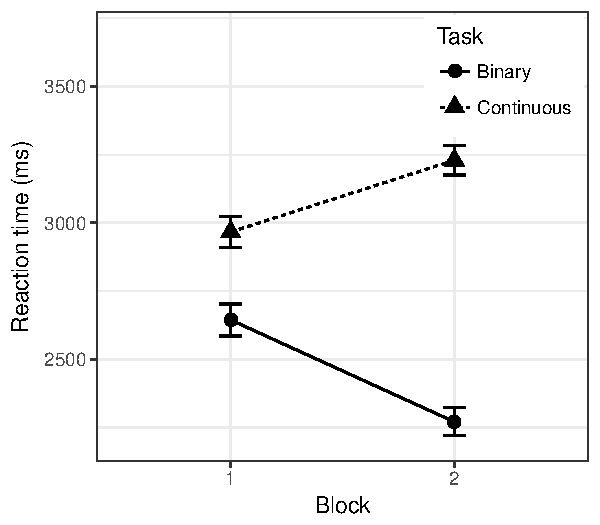
\includegraphics{images/RTorderEffects.pdf}
	\caption{Mean reaction times. Error bars are within-subject difference-adjusted confidence intervals \protect\cite{Baguley2012}.}
	\label{figure:RTblockGraph}
\end{figure}

There was a significant variance in reaction time intercepts across participants, $SD=1114.18$ (95\% CI: 900.45, 1378.63), $\chi^2(1)=1375.60$, $p<.001$. Additionally, slopes based on absolute difference in attention significantly varied across participants, $SD=556.09$ (95\% CI: 275.62, 1121.96), $\chi(2)=9.66$, $p=.008$. As did the slopes based on absolute difference in value, $SD=90.54$ (95\% CI: 52.81, 155.24), $\chi(3)=15.26$, $p=.002$. Therefore, the final model included main effects of task, attention and value, with random effects of attention and value. 
	

% Table created by stargazer v.5.2.2 by Marek Hlavac, Harvard University. E-mail: hlavac at fas.harvard.edu
% Date and time: Tue, Jun 04, 2019 - 15:10:04
\begin{table}[t] \centering 
  \caption{Summary of coefficients of model predicting reaction time} 
  \label{table:rtModel} 
\begin{tabular}{@{\extracolsep{5pt}}lc} 
\\[-1.8ex]\hline 
\hline \\[-1.8ex] 
 & \multicolumn{1}{c}{\textit{Dependent variable:}} \\ 
\cline{2-2} 
\\[-1.8ex] & rt \\ 
\hline \\[-1.8ex] 
 Task & 299.238 ($-$313.417, 911.894) \\ 
  $\vert\Delta_A\vert$ & $-$801.637$^{**}$ ($-$1,415.806, $-$187.468) \\ 
  $\vert\Delta_V\vert$ & $-$90.223$^{**}$ ($-$175.690, $-$4.757) \\ 
  Task : $\vert\Delta_A\vert$ & $-$143.654 ($-$977.778, 690.469) \\ 
  Task : $\vert\Delta_V\vert$ & 11.538 ($-$103.462, 126.537) \\ 
  $\vert\Delta_A\vert$ : $\vert\Delta_V\vert$ & 12.598 ($-$282.011, 307.207) \\ 
  Task : $\vert\Delta_A\vert$ :  $\vert\Delta_V\vert$ & 120.222 ($-$274.293, 514.737) \\ 
  Constant & 2,989.224$^{***}$ (2,547.009, 3,431.439) \\ 
 \hline \\[-1.8ex] 
Observations & 2,557 \\ 
Log Likelihood & $-$21,556.920 \\ 
Akaike Inf. Crit. & 43,135.830 \\ 
Bayesian Inf. Crit. & 43,200.140 \\ 
\hline 
\hline \\[-1.8ex] 
\textit{Note:}  & \multicolumn{1}{l}{\footnotesize $\vert\Delta_A\vert$ = absolute attention difference; $\vert\Delta_V\vert$ = absolute value difference; } \\ 
\end{tabular} 
\end{table} 


Table~\ref{table:rtModel} contains the coefficients and 95\% confidence intervals for the fixed effects in the full reaction time model (see Figure~\ref{figure:RTattentionValueGraph}). In summary, reaction times were significantly predicted by difference in attention, $t(2499)=2.11$, $SE=334.42$, $p=.035$. The greater the difference in amount of attention between the two options, the faster the participant responded. There was also a marginal effect of difference in value, $t(2499)=1.71$, $SE=45.69$, $p=.088$. The greater the difference in value between the choices, the faster participants responded. The main effect of task, the two-way and three-way interactions did not reach significance ($p>=0.316$). 

\begin{figure}
	\centering
	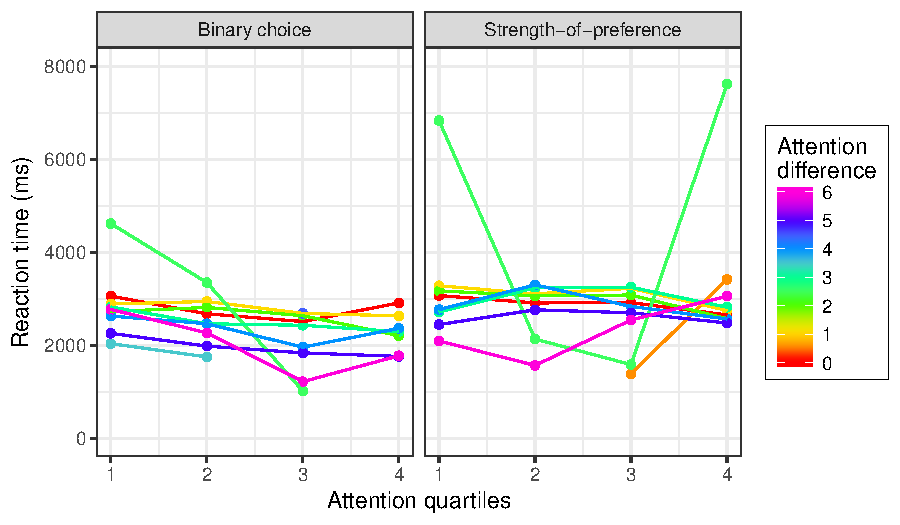
\includegraphics{images/RTattentionValueGraph}
	\caption{}
	\label{figure:RTattentionValueGraph}
\end{figure}

\subsection{Choice}
To consider a mixed effects model of choice, we recoded the responses given in the continuous task as binary. Other ways of completing this analysis, which attempted to take into account the additional information available in the continuous tasks (such as linear probability models), found similar results. 

There was no interaction between task and order on choice, $p=.766$. Additionally, a main effects analysis found the four-way interaction was not significant, $p=.999$. Therefore, in the following we disregard order as a main effect and include data from both tasks. 

There was a significant random effect of difference in attention on choice, $\chi^2(1)=1791.02$, $p<.001$. There was also a random effect of difference in value on choice, $\chi^2(1)=1341.70$, $p<.001$. A random effect of task did not add additional information, $\chi^2(3)=0.46$, $p=.928$. Therefore, the final model included fixed effects of task, attention and value, with random effects of attention and value.


% Table created by stargazer v.5.2.2 by Marek Hlavac, Harvard University. E-mail: hlavac at fas.harvard.edu
% Date and time: Tue, May 28, 2019 - 18:03:45
\begin{table}[!b] \centering 
  \caption{Summary of coefficients of model predicting choice} 
  \label{table:choiceModel} 
\begin{tabular}{@{\extracolsep{5pt}}lc} 
\\[-1.8ex]\hline 
\hline \\[-1.8ex] 
 & \multicolumn{1}{c}{\textit{Dependent variable:}} \\ 
\cline{2-2} 
\\[-1.8ex] & recodedResponse \\ 
\hline \\[-1.8ex] 
 Task & $-$0.013 ($-$0.178, 0.152) \\ 
  Attention & 5.677$^{***}$ (4.814, 6.540) \\ 
  Value & 0.891$^{***}$ (0.769, 1.014) \\ 
  Task:Attention & 0.574 ($-$0.242, 1.389) \\ 
  Task:Value & 0.022 ($-$0.084, 0.128) \\ 
  Attention:Value & 0.060 ($-$0.281, 0.401) \\ 
  Task:Attention:Value & $-$0.112 ($-$0.618, 0.395) \\ 
  Constant & 0.017 ($-$0.115, 0.150) \\ 
 \hline \\[-1.8ex] 
Observations & 5,115 \\ 
Log Likelihood & $-$1,881.974 \\ 
Akaike Inf. Crit. & 3,785.949 \\ 
Bayesian Inf. Crit. & 3,857.888 \\ 
\hline 
\hline \\[-1.8ex] 
\textit{Note:}  & \multicolumn{1}{r}{$^{*}$p$<$0.1; $^{**}$p$<$0.05; $^{***}$p$<$0.01} \\ 
\end{tabular} 
\end{table} 
 

Table~\ref{table:choiceModel} contains the coefficients and 95\% confidence intervals for the fixed effects in the full choice model. Choice was significantly predicted by attention, $t(1)=12.89$, $SE=0.44$, $p<.001$, and value, $t(1)=14.28$, $SE=0.06$, $p<.001$. The main effect of task, as well as two- and three-way interactions did not reach significance ($p>=.168$).

\section{Discussion}

\section{Open Practices Statement}
The analysis was pre-registered at \url{AsPredicted.org/19698}. The data and analysis of this experiment is available in the Open Science Framework \url{https://osf.io/xfc8a/}. 
% TODO Double check links are correct. 

\newpage
\bibliographystyle{apacite}
\bibliography{references}

\end{document}